\documentclass[11pt]{article}
\usepackage[sc]{mathpazo} %Like Palatino with extensive math support
\usepackage{fullpage}
\usepackage[authoryear,sectionbib,sort]{natbib}
\linespread{1.7}
\usepackage[utf8]{inputenc}
\usepackage{lineno}
\usepackage{titlesec}

\usepackage{graphicx,float}
% for setting up equations
\usepackage{amsmath}
\usepackage[usenames,dvipsnames]{xcolor}
\usepackage{gensymb}

\titleformat{\section}[block]{\Large\bfseries\filcenter}{\thesection}{1em}{}
\titleformat{\subsection}[block]{\Large\itshape\filcenter}{\thesubsection}{1em}{}
\titleformat{\subsubsection}[block]{\large\itshape}{\thesubsubsection}{1em}{}
\titleformat{\paragraph}[runin]{\itshape}{\theparagraph}{1em}{}[. ]\renewcommand{\refname}{Literature Cited}

\graphicspath{{/Users/jm200/Library/CloudStorage/Dropbox/Miller Lab/github/ELVI-endophyte-density/Figure/}}
\newcommand{\tom}[2]{{\color{red}{#1}}\footnote{\textit{\color{red}{#2}}}}
\newcommand{\jacob}[2]{{\color{blue}{#1}}\footnote{\textit{\color{blue}{#2}}}}

%%%%%%%%%%%%%%%%%%%%%
% Line numbering
%%%%%%%%%%%%%%%%%%%%%
%
% Please use line numbering with your initial submission and
% subsequent revisions. After acceptance, please turn line numbering
% off by adding percent signs to the lines %\usepackage{lineno} and
% to %\linenumbers{} and %\modulolinenumbers[1] below.
%
% To avoid line numbering being thrown off around math environments,
% the math environments have to be wrapped using
% \begin{linenomath*} and \end{linenomath*}
%
% (Thanks to Vlastimil Krivan for pointing this out to us!)

\title{Variation in the demographic effects of grass-endophyte symbiosis along an aridity gradient }
% This version of the LaTeX template was last updated on
% July 16, 2024.

%%%%%%%%%%%%%%%%%%%%%
% Authorship
%%%%%%%%%%%%%%%%%%%%%
% Please commet out authorship information while your paper is under review. 
% You will need to add this information back in to your final files after
% acceptance.

\author{Jacob K. Moutouama$^{1,\ast}$ \\ 
Julia Martin$^{1}$ \\ 
Ulisses Rizo$^{1}$\\
Malcolm Sherwood$^{1}$\\
Emily Chong$^{1}$\\
Dajanae Pearson$^{1}$\\
Alexandra Jimenez Martín$^{1}$\\
Josh Fowler$^{2}$\\
Ali Campbell$^{1}$\\
Chris Oxley$^{1}$\\
Karl Schrader$^{1}$\\
Tom E.X. Miller$^{1}$\\}

\date{}

\begin{document}

\maketitle

\noindent{} 1. Program in Ecology and Evolutionary Biology, Department of BioSciences, Rice University, Houston, TX USA;

\noindent{} 2. University of Miami, Department of Biology, Miami, Florida;

\noindent{} $\ast$ Corresponding author; e-mail: jmoutouama@gmail.com.

%\noindent{} $\dag$ Deceased.

\bigskip

%\textit{Manuscript elements}: Figure~1, figure~2, table~1, appendix~A (for print; including figure~A1, figure~A2, and table~A1), supplemental PDF. Figure~2 is to print in color.

\bigskip

%\textit{Keywords}: Examples, model, template, guidelines.

\bigskip

\textit{Manuscript type}: Article. %Or note, natural history miscellany note, comment, reply, invited symposium, featured topic, or historical perspective.

\bigskip

%\noindent{\footnotesize Prepared using the suggested \LaTeX{} template for \textit{Am.\ Nat.}}

\linenumbers{}
\modulolinenumbers[1]

\newpage{}

\section*{Abstract}

\newpage{}

\section*{Introduction}

% The journal does not have numbered sections in the main portion of
% articles. Please refrain from using section references (à la
% section~\ref{section:CountingOwlEggs}), and refer to sections by name
% (e.g. section ``Counting Owl Eggs'').

Plant-microbe symbioses are widespread and ecologically important. 
These interactions are famously context-dependent, where the direction and strength of the interaction outcome depends on the environment in which it occurs \citep{fowler2023geographic,hoeksema2015context, bronstein1994conditional}.
Plant-microbe  interactions that are beneficial under stressful conditions  may become parasitic under benign conditions \citep{giauque2019endophyte}.
Under biotic stress (e.g., herbivory), endophyte symbiosis can benefit host plants by facilitating the production of secondary compounds that deter feeding or exert direct toxicity, thereby reducing insect growth, survival, and oviposition \citep{atala2022fungal,bastias2017epichloe,vega2008insect}.
Similarly under abiotic stress (e.g., drought), symbionts can increase their host tolerance  \citep{clay2002evolutionary}.
However, in many plant-microbe interactions, host protection is not guaranteed solely by the presence of a symbionts; rather, the density of the symbiont can determine the effectiveness of this protection \citep{laughton2014combined}. 
Higher endophyte densities may lead to increased resource exploitation by the symbiont, potentially imposing costs on the host, such as reduced growth or reproduction \citep{faeth2009asexual}.
%This cost is often manifested by a reduction in host biomass or reproductive success \citep{faeth2009asexual}, particularly under harsh abiotic conditions \citep{cui2024review}. 
%Ultimately, these context-dependent costs and benefits may underlie the observed distribution of host species.

Context dependence raises the hypothesis that plant-microbe interactions are likely to vary across environmental gradients, from range core to range edge, with significant implications for host range expansion. If microbial symbiosis provides greater benefits under environmental stress, then symbionts could enhance the suitability of range-edge environments, potentially extending host range limits \citep{allsup2023shifting,rudgers2020climate}.
For instance, fungal endophytes improve the survival of \emph{Bromus laevipes}  populations in dry conditions, increasing their drought resistance at the range edge and thereby extending the species' geographic range \citep{david2019soil,afkhami2014mutualist}.
Even if the symbiont does not directly improve host survival, it may still enhance host population growth over time by increasing relative growth and reproduction, potentially offsetting the negative effects of lower survival rates \citep{yule2013costs}.
Conversely, if microbial symbiosis is costly for the host at range edge, symbionts could constrain host range \citep{benning2021microbes,benning2021plant,bennett2022costs}.
%Mutualist limitation reduces population fitness and therefore limits range expansion in \emph{Medicago polymorpha} populations \citep{lopez2021microbial}. 
Although context dependence, along with spatiotemporal variations in abiotic environmental conditions may reduce the effectiveness of the benefits provided by the symbiont to the host species, our understanding of the mechanisms that alter host-symbiont interactions across species geographic range remains limited.

Ecological studies of plant-microbe symbiosis typically examine interactions from the plant’s perspective and rarely manipulate symbiont frequency to explore how symbiont response to environmental variation might translate to effect on host demographic performance across host's range.
Symbionts  promotes their own fitness by influencing their host's life history traits and resistance to abiotic and biotic stress \citep{kazenel2015mutualistic,giauque2019endophyte,saikkonen1998fungal}. 
Therefore overlooking the role of symbionts and their potential cascading effects on the eco-evolutionary population dynamics of host species  could lead to inaccurate prediction of host response to global change. 
Moreover, studies on plant-microbe symbiosis often fail to account for  the synergistic effects of abiotic and biotic factors on host dynamics across species ranges.
Finally, studies of plant-microbe symbiosis have relied on methods  such as inoculating sterile soil \citep{peacher2020inoculum}, excluding endophyte fungal hyphae using fine mesh or rotating cores \citep{chung2019connecting}, and applying fungicide \citep{bennett2022costs}. 
While valuable, these approaches are often challenging to implement in field settings or on large scales.
As a result, the mechanisms by which symbionts drive host range limitation and expansion are poorly understood, hindering our understanding of the potential cascading effects of symbionts on eco-evolutionary species demography and  range limitation in the context of global change.
%Symbionts are promoting their own selfish fitness by manipulating their hosts' life history traits or resistance to stresses caused by abiotic and biotic variation \citep{kazenel2015mutualistic,giauque2019endophyte,saikkonen1998fungal}. 
%% Plant host–promoted tolerance to these stresses by the fungi may come at a cost.  
%Therefore overlooking the role of symbionts and their potential cascading effects on the eco-evolutionary population dynamics of host species  could lead to inaccurate prediction of host response to current global change. 
% For instance fungal endophyte can reduce plant vital rates (e.g survival) but increase population fitness \citep{rudgers2012there,ahlholm2002vertically}. 

%Understanding how symbiotic interactions are likely to facilitate host persistence in changing environments requires an investigation of the synergistic effects of biotic, abiotic stressors and endophyte presence on individual demographic performance (survival, growth and reproduction) and how that effect can be translated at a population level \citep{bruno2003inclusion,de2006fungal}. 
%One of the best ways to perform that investigation is to use common garden experiments along climatic gradient \citep{schwinning2022common}.
%These common gardens experiments allow the manipulation of variation of biotic and abiotic factors that are likely to change with climate change (eg. temperature, precipitation, endophyte prevalence) and measured species response of such a variation.  

Working across a precipitation gradient in the south-central US, we investigated  how the demographic effects of endophyte symbiosis varied from core to edge of the host range.
To answer these questions, we studied the symbiotic association between  cool-season grass species (\emph{Agrostis hyemalis}, \emph{Elymus virginicus} and \emph{Poa arachnifera}) and its vertically transmitted fungal symbiont Epichloë elymi. \jacob{[Describe ecology and natural history of grass-endophyte interactions]}{I am not sure If we need this}.
Our experiment was design to test the following \jacob{hypotheses}{ I need to update these hypotheses by adding the herbivory effect} :
\begin{enumerate}
\item We hypothesized that stress associated with aridity and low precipitation would strengthen the plant-fungal mutualism, such that the fitness benefits of endophyte symbiosis are maximized at the range edge. 
\item We hypothesized that fungal growth in planta varied from range core to range edge. If endophyte growth is limited by host photosynthesis, then environments that are stressful for hosts may correspond to poor endophyte growth. Alternatively, if active regulation by the host is required to keep symbionts “in check”, then environments that are stressful for hosts may correspond to high endophyte growth.
\end{enumerate}

%--------------------------------------------------------------------
\section*{Materials and methods}
\subsection*{Study species}
\emph {Elymus virginicus} (Poaceae) is a cool season perennial grass native to woodland and prairie habitats of eastern North America \citep{shaw2011guide}. 
The westernmost range limits of this species correspond to the longitudinal aridity gradient in the central and southern Great Plains (fig. \ref{fig:site}). 
Throughout its range, the species is  symbiotic with the seed-transmitted fungal endophyte (Epichloë spp.) \citep{rudgers2009benefits}. 
Across natural populations in Texas, endophyte prevalence (fraction of plants that are endophyte-symbiotic) in \emph {Elymus virginicus}  ranged from 10\% to 100\%, with a mean of 53\% \citep{sneck2017variation}. 
Fungal genotyping indicated that the endophytes are capable of synthesizing secondary compounds such as peramine, loline, and ergot alkaloids, which may confer resistance against drought and herbivory \citep{beaudry1951seed}.
In addition, the species is capable of both self-pollination and outcrossing \citep{church1958artificial}. 

\begin{figure}[h!]
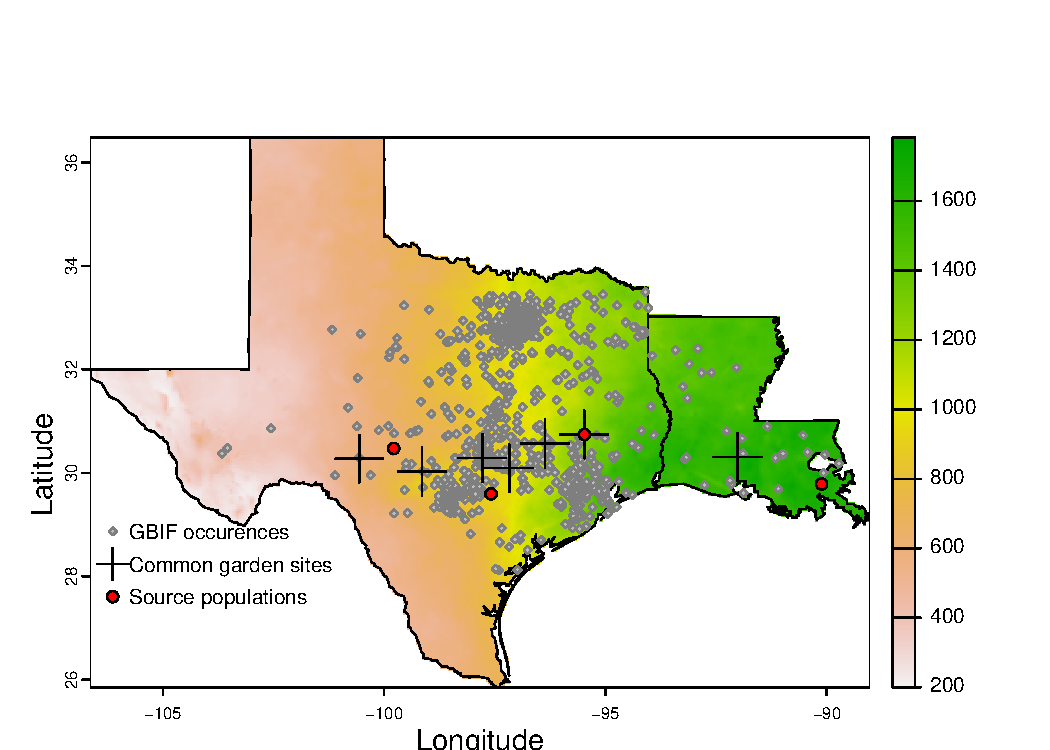
\includegraphics[width=1\textwidth]{clim_map_v1.pdf}
\caption{Distribution of common garden sites across the longitudinal aridity gradient in the central and southern Great Plains. 
Red dots represent the locations of source populations, while grey dots represent the GBIF locations of the species across the study area.}
\label{fig:site}
\end{figure}

\subsection*{Study design}
\paragraph {Experimental Design} 
To understand the demographic effects of endophyte symbiosis from core to edge of the host range, we established  common gardens at 7 sites across the geographic range of \emph {Elymus virginicus} (fig. \ref{fig:site}).
Experimental sites spanned an aridity gradient (temperature gradient).
Common gardens were established in 8 plots per site. 
Plots were 1.5m * 1.5m and the area was tilled of existing vegetation to control for native plant competition.
Plots were also selected in shaded areas under tree canopy or near shrubs to mimic the natural environmental of the species.
In each plot,  we planted 15 individuals  of \emph{E. virginicus} approximately 15 cm deep in an evenly spaced 4*4 grid pattern, with positions randomly assigned. 
For each plot, we randomly assigned a starting endophyte frequency  \jacob{(80\%, 60\%, 40\%, 20\%)}{Do we need a schematic of one replicate
of the experimental design?} and herbivory treatment (herbivores exclusion and herbivores accessibility). 
%Here, the endophyte frequency represents the percentage of  \emph{E. virginicus} individuals that have a symbiont ($E^+$).
We ensured that all plots had comparable quantities of source populations.
After establishing the plots, we watered the plants and recorded initial tiller counts, flowering status and plot position,  endophyte status, source population of each individual plant. 
For herbivory exclusion plots, we enclosed them with 1.2m tall mesh fencing to prevent browsing by vertebrate herbivores and sprayed the plots with insecticide. 
For herbivores accessibility plots (control treatment), we half enclosed the plots with the mesh netting.
We stationed one HOBO MX2307 data logger at each site to collect temperature and volumetric water content in the soil every hour. 

\paragraph {Source populations and Identification of individual endophyte status} 
Plants used  in the common garden experiment were derived from natural populations throughout the native range in the south-central US (fig.\ref{fig:site}, \jacob{Table X}{We need this table  in the Appendix}). 
At each of these natural populations we collected seeds. 
Some of the seeds of \emph{E. virginicus} were heat treated to produce endophyte negative plants ($E^-$) . 
To do so, we placed these seeds  in a drying oven set at 60°C for approximately five days (120 hours). 
While this method eliminates the endophytes from all individuals, it does not affect seed viability. 
All seeds (both heat-treated and non-heat-treated) were planted in the Rice University greenhouse.
Seedlings were regularly fertilized every two weeks. 
The seedlings were then vegetatively propagated to produce enough individuals for your experiment (N = 840).
Before planting in the field, we confirmed the endophyte status ($E^+$ or $E^-$) of all  seedlings using either microscopy or an immunoblot assay. 
This was necessary due to the varying success of the heat treatment and differences in the prevalence of endophytes between the natural populations. 
Leaf tissues were stained with aniline blue lactic acid and viewed under a compound microscope at 200x-400x to identify fungal hyphae. 
The immunoblot assay (Phytoscreen field tiller endophyte detection kit, Agrinostics Ltd. Co.) uses monoclonal antibodies that target proteins of Epichloë spp. and chromagen to visually indicate presence or absence. Both methods yield similar detection rates.  
%The vegetatively cloned plants were distributed across all sites intentionally to allow for comparison of endophyte hyphae densities.

\subsection*{Climatic data}
To characterize the stress gradient with respect to  climatic conditions, we collected the hourly temperature and soil moisture at each site using the HOBO MX2307 data loggers. We used this hourly variable to calculate the daily mean temperature (°C) and soil moisture (\%)(fig. \ref{fig:climate}). 
\jacob{We calculated the mean soil moisture and the coefficient of variation from the time the plants were placed on the ground to the time we collected demographic data}{I will change this  later}. 
The coefficient of variation of soil moisture was estimated to capture season variability in climatic data \citep{medvigy2012trends,meshram2017long}. 

\begin{figure}[h!]
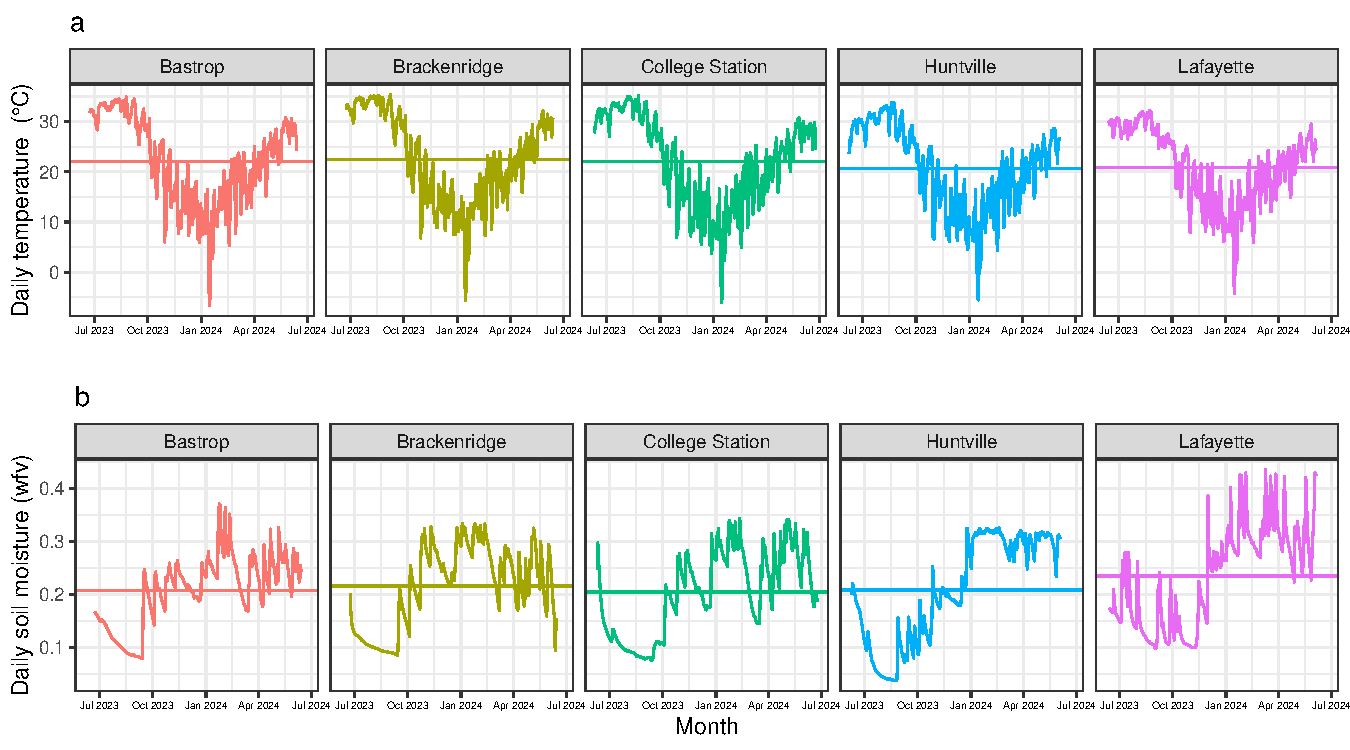
\includegraphics[width=1\textwidth]{climatesite.pdf}
\caption{Climate variation  across common garden sites. 
(a) Daily temperature, estimated from average hourly data collected by  HOBO data loggers. 
(b) Daily  soil moisture, estimated  from average hourly data  collected by  HOBO data loggers. 
}
\label{fig:climate}
\end{figure}

\subsection*{Demographic data}
We collected demographic data including survival, growth, and reproduction during June 2023, which coincided with the flowering season of \emph{E. virginicus}. 
On each individual, survival of plants was recorded as a binary (death or alive) and the size of the plant was recorded as the number of living tillers, indicated by the presence of green coloration. 
We recorded the number of inflorescences per plant and the number of spikelets on up to three inflorescences from three reproducing plants.
We limited the spikelets count to three reproducing tillers per plot due to the time consuming nature of this measurement process. 
We used the number of spikelets for these three tillers to estimate the number the average number of spikelets per plants.

%\subsection*{Endophyte density measurements}
%We collected leaf samples from E+ genotypes that were clonally replicated across two or more sites to quantify endophyte hyphal density and test its associations with host genotype and environmental factors. 
%Relying on clonally replicated genotypes for this analysis allowed us to observe the same genetic individuals in different environments, and partition variation in symbiont density between genetic and environmental sources. 
%
%There were seven unique genotypes of E+ hosts (three PALM, three JLP, one SHS) that were clonally replicated across two or more experimental sites. 
%We collected leaf samples from clonal replicates of these genotypes at up to five sites (excluding COL and SON, where no samples were taken) at the time of the demographic census.
%Samples were taken opportunistically based on survival status and size (we avoided leaf collection from small individuals with few leaves that were vulnerable to mortality).
%We collected 20 leaf samples in total, consisting of one genotype replicated at five sites, three genotypes replicated at three sites, and three genotypes replicated at two sites. 
%
%Samples were placed in a cold cooler in the field and then stored in a -20 freezer until processing.
%In the lab, we examined sections of inner leaf sheath for hyphal density. 
%For each sample, four “peels” of the leaf sheath were placed on a single gridded glass slide (including xmm cells), stained with an aniline blue-lactic acid solution, and viewed under a light microscope at X magnification, following methods in \textcolor{violet}{Sneck et al. 2019}. 
%We randomly sub-sampled cells on the gridded slide, skipping those with less than 25\% leaf peel coverage, until we reached 10 cells for each sample, which amounted to a subsample totaling up to 12mm² per leaf.
%We took digital images of each grid cell. 
%Using ImageJ, we set the scale using the microscope reticle to measure the visible area of the leaf peel within the cell and the total length of the hyphae fragments within the leaf peel.
%This yielded an estimate of endophyte density in the units of length (mm) per area (mm2). 

\subsection*{Models building and models selection}
To assess how stress associated with aridity  affect plant-fungal mutualism, we developed four candidates models for each vital rate (survival, growth, flowering, fertility). 
Each vital rate was modeled with  the  grand mean intercept ($\beta_{0}$), slopes for  variation in each covariate ($\beta_{1}$...$\beta_{3}$) as well as the interaction between covariates ($\beta_{4}$...$\beta_{6}$): 
Each model includes normally distributed random effects for site-to-site  variation ($\phi \sim N(0,\ \sigma_{site})$), plot to plot variation ($\rho \sim N(0,\ \sigma_{site})$), and source-to-source variation that is related to the  provenance of the transplants used to establish the common garden ($\omega \sim N(0,\ \sigma_{source})$) (Eq.\ref{eq:candidates}).
\begin{align}\label{eq:candidates}
\begin{split}
model1 = \beta_{0} + \beta_{1}T_{mean}  + \beta_{2}E + \beta_{3}H + \beta_{4}E*T_{mean} + \beta_{5}H*E +  \beta_{6}H*T_{mean} + \phi + \omega + \rho  \\ 
model2  = \beta_{0} + \beta_{1}T_{CV}  + \beta_{2}E + \beta_{3}H + \beta_{4}E*T_{CV} + \beta_{5}H*E +  \beta_{6}H*T_{CV} +  \phi + \omega + \rho  \\
model3  = \beta_{0} + \beta_{1}M_{mean}  + \beta_{2}E + \beta_{3}H + \beta_{4}E*M_{mean} + \beta_{5}H*E +  \beta_{6}H*M_{mean} + \phi + \omega + \rho \\
model4  = \beta_{0} + \beta_{1}M_{CV}  + \beta_{2}E + \beta_{3}H + \beta_{4}E*M_{CV} + \beta_{5}H*E +  \beta_{6}H*M_{CV} + \phi + \omega + \rho 
\end{split}
\end{align}
 
We modeled survival using a  Bernoulli distribution, growth with a Gaussian distribution, flower with a negative binomial and fertility (number of spikelet) with a negative binomial distribution.
To check whether the fitted models are  compatible with the observed data, we used the posterior predictive checks \citep{gelman2000diagnostic,berkhof2000posterior}. 
All models  do a good job of capturing relevant aspects of the data, such as means, standard deviations, and quantiles (fig.\ref{sup:ppc_surv}, fig.\ref{sup:ppc_growth}, fig.\ref{sup:ppc_spikelet}, fig.\ref{sup:ppc_flowering}).

\jacob{To select the best model for each vital rate, we compared the four models using the leave-one-out cross-validation (LOOCV)} {I need to add something about  difference in  models} \citep{vehtari2017practical}. 
LOOCV combines both validation and training methods. 
In this approach, one observation is used for validation while the training set consists of n-1 observations. 
This process is repeated for each observation, resulting in n estimated models \citep{silva2024robust}. 
The estimate of test error from LOOCV is calculated by averaging the errors across these n models (Eq.\ref{eq:Loo}).
\begin{align}\label{eq:Loo}
\begin{split}
CV_{n}=\frac {1}{n} \sum^{n}_{i=1}{(y_{I}-\hat{y}_{I})^2}
\end{split}
\end{align}

All models were performed in R \citep{RCoreTeam} and Stan \citep{Rstan}.
%%%%%%%%%%%%%%%%%%%%%
% Acknowledgments
%%%%%%%%%%%%%%%%%%%%%
% You may wish to remove the Acknowledgments section while your paper 
% is under review as the Acknowledgments may reveal your identity.
% If you remove this section, you will need to add it back in to your
% final files after acceptance.
\section*{Results}
\begin{table}[H]
\caption{Candidate models of  \emph{E. virginicus} vital rates (growth, flowering, spikelet and survival).}
\label{Table:models}
\bigskip{}
\centering
\begin{tabular}{llll}\hline
			    Vital rate   &      Model   &     $\Delta$elpd  &  $\Delta$se     \\ \hline
			 \textbf{Survival} &    \textbf{model3}   &     \textbf{0.0} &     \textbf{ 0.0}    \\
			Survival &     model2  & -0.5 &   0.5       \\
			Survival &   model4    & -0.9    &   0.9\\
			Survival & model1 & -2.2 & 1.9  \\
		     \textbf{Growth} &   \textbf{model2}&  \textbf{0.0} &  \textbf{0.0} \\
		    Growth & model4 & 0.0 &  0.8 \\
		    Growth & model3 & -0.3 &  0.4\\
		    Growth  &  model1& -0.4 & 0.4\\
		     \textbf{Flowering} &   \textbf{model2}&  \textbf{0.0}  &  \textbf{0.0}  \\
		    Flowering & model4 & -4.3 &  1.0\\
		    Flowering & model3 & -6.5 &  1.4\\
		     Flowering & model3 & -6.5 &  1.4\\
		    		     \textbf{Spiket} &   \textbf{model2}&  \textbf{0.0} &  \textbf{0.0}  \\
		    Spiket & model3 & -0.5 &  0.6\\
		    Spiket & model1 & -0.7&  1.2\\
		    Spiket  &  model4 & -1.2 & 1.2\\\hline			    				 			     			     
\end{tabular}
\end{table}

\begin{figure}[H]
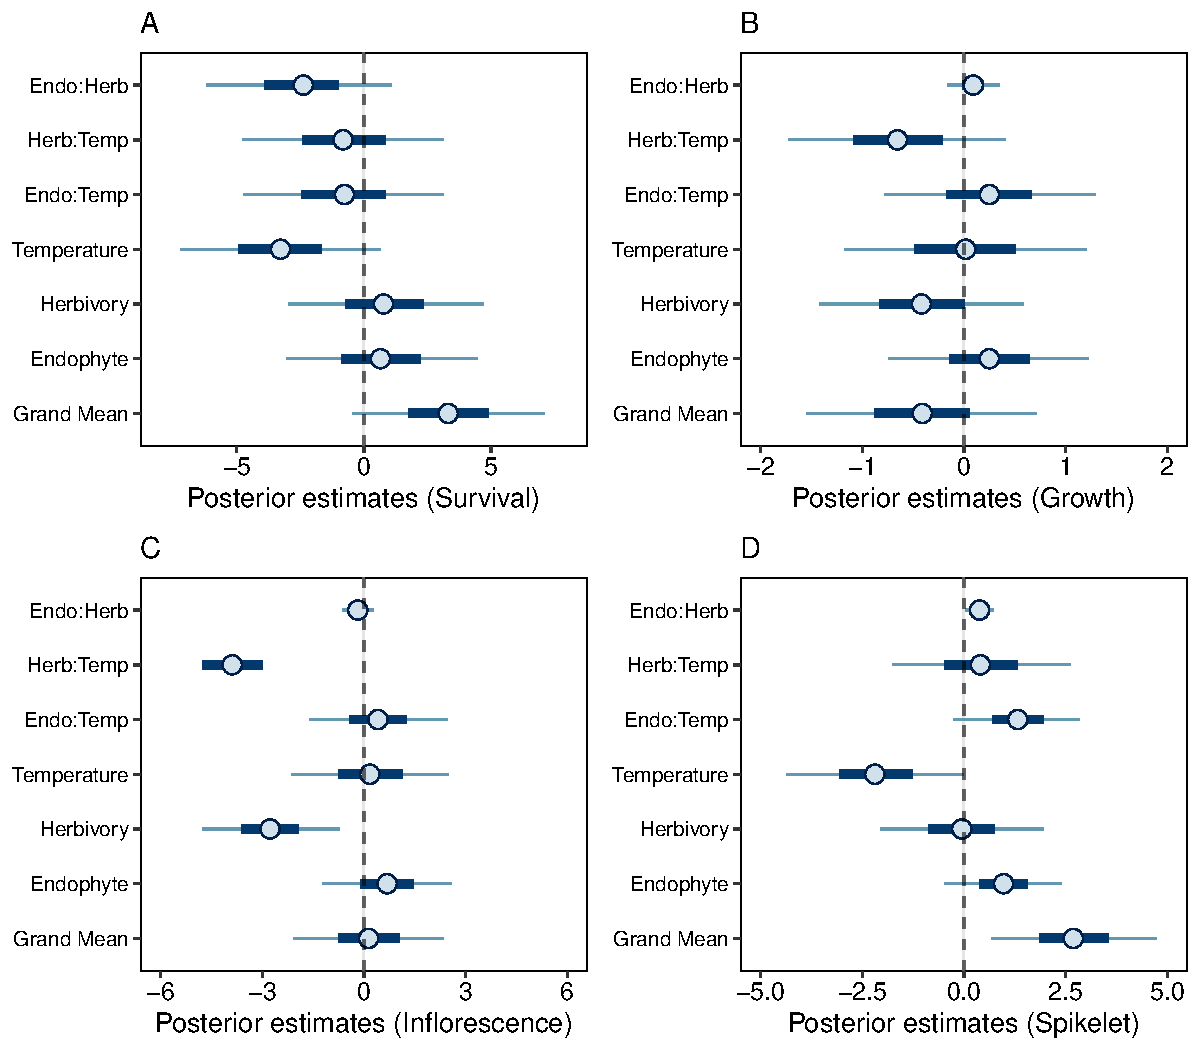
\includegraphics[width=1\textwidth]{Posterior_mean.pdf}
\caption{Posterior mean estimates for each vital rate. 
(a) Daily temperature, estimated from average hourly data collected by  HOBO data loggers. 
(b) Daily  soil moisture, estimated  from average hourly data  collected by  HOBO data loggers. 
}
\label{fig:climate}
\end{figure}

\begin{figure}[H]
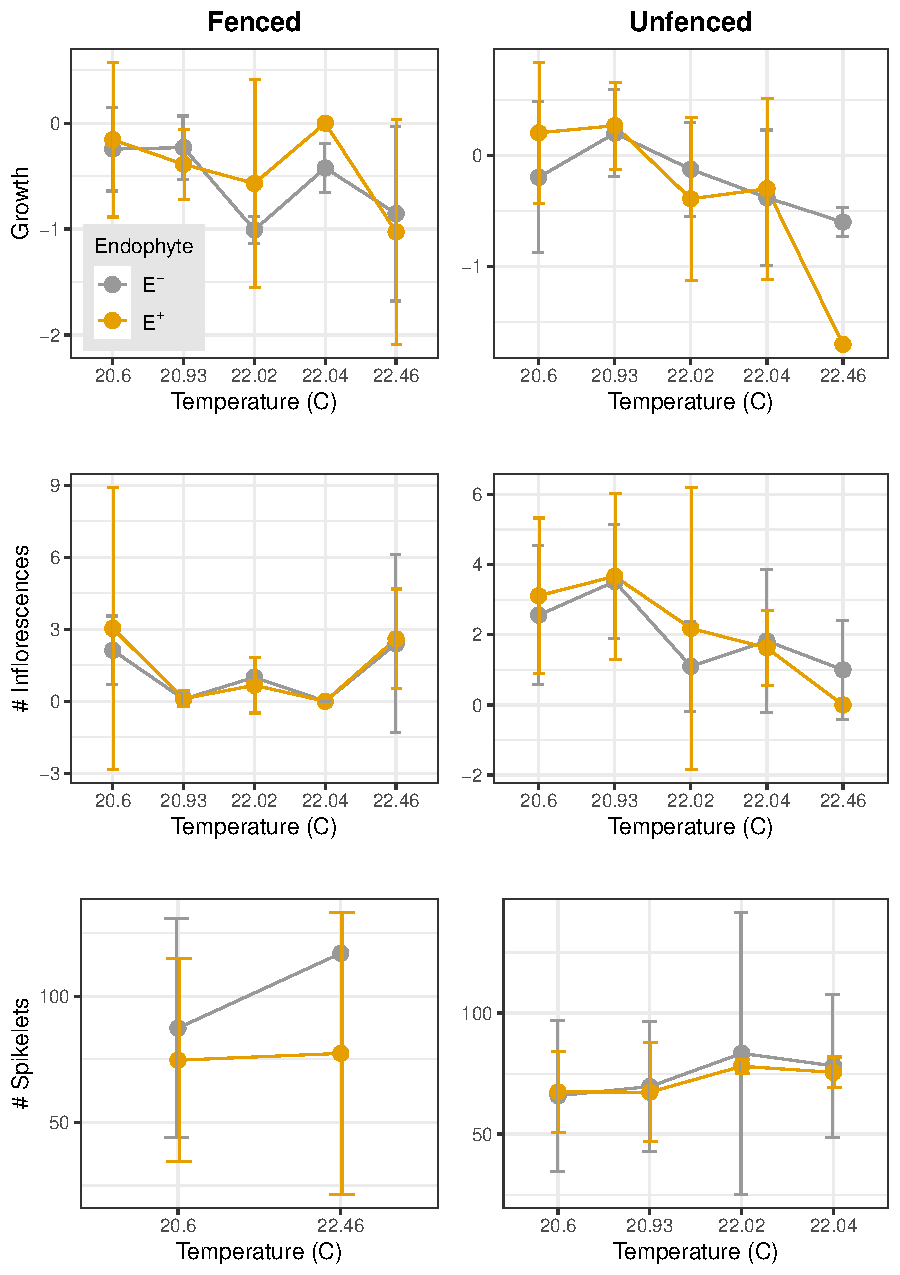
\includegraphics[width=0.9\textwidth]{Fig_temp_mean.pdf}
\caption{Variation in vital rates across a temperature gradient.
}
\label{fig:vital}
\end{figure}


\section*{Acknowledgments}


%%%%%%%%%%%%%%%%%%%%%
% Statement of Authorship
%%%%%%%%%%%%%%%%%%%%%
% This section should also be commented out while your MS is undergoing
% double-blind review. The specifics should of course be adapted to
% your paper, but the paragraph below gives some hints of possible
% contributions.

\section*{Statement of Authorship}

\section*{Data and Code Availability}
\newpage{}	
\section*{Appendix A}
\renewcommand{\thefigure}{A\arabic{figure}}
\setcounter{figure}{0}
	
\renewcommand{\thetable}{A\arabic{table}}
\setcounter{equation}{0}  % reset counter 
\setcounter{figure}{0}
\setcounter{table}{0}

\begin{figure}[h!]
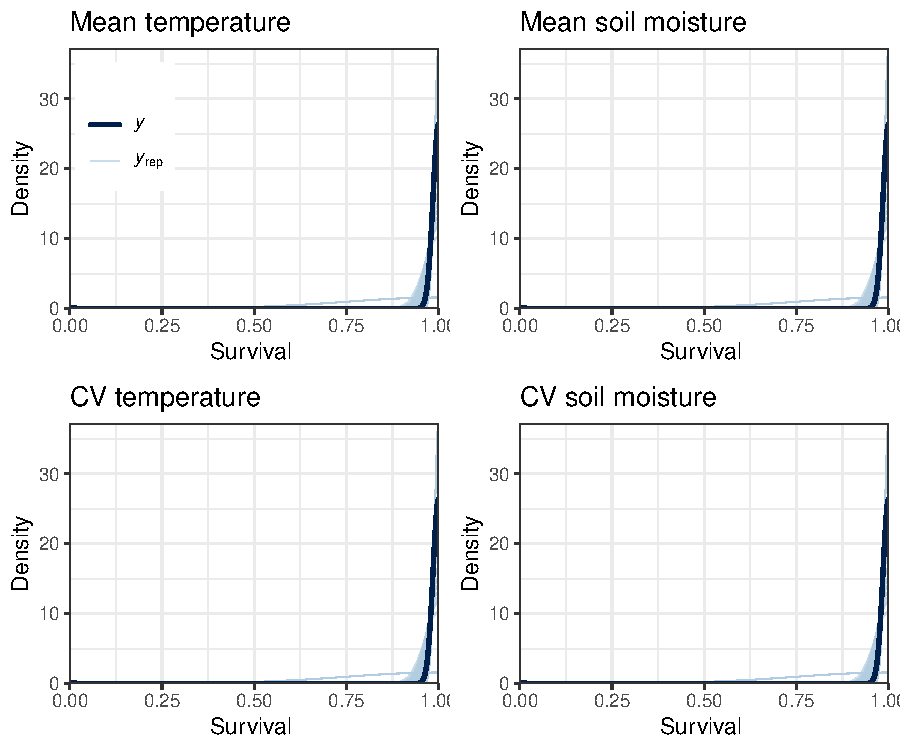
\includegraphics{PPC_survival}
\caption{Comparison of the observed survival data with the posterior predictions from the survival models for each climate variable}
\label{sup:ppc_surv}
\end{figure}
\clearpage

\begin{figure}[h!]
\includegraphics{PPC_growth}
\caption{Comparison of the observed growth data with the posterior predictions from the growth models for each climate variable}
\label{sup:ppc_growth}
\end{figure}
\clearpage

\begin{figure}[h!]
\includegraphics{PPC_spikelet}
\caption{Comparison of the observed spikelet data with the posterior predictions from the spikelet models for each climate variable}
\label{sup:ppc_spikelet}
\end{figure}
\clearpage

\begin{figure}[h!]
\includegraphics{PPC_flowering}
\caption{Comparison of the observed  flowering data with the posterior predictions from the flowering  models for each climate variable}
\label{sup:ppc_flowering}
\end{figure}
\clearpage


%%%%%%%%%%%%%%%%%%%%%
% Bibliography
%%%%%%%%%%%%%%%%%%%%%
% You can either type your references following the examples below, or
% compile your BiBTeX database and paste the contents of your .bbl file
% here. The amnatnat.bst style file should work for this---but please
% let us know if you run into any hitches with it!
%
% If you upload a .bib file with your submission, please upload the .bbl
% file as well; this will be required for typesetting.
%
% The list below includes sample journal articles, book chapters, and
% Dryad references.
\newpage{}
\bibliographystyle{amnatnat}
\bibliography{ELVI}

\newpage{}

\newpage{}

% Figure legends for any print appendices you might have.



%%%%%%%%%%%%%%%%%%%%%
% Videos
%%%%%%%%%%%%%%%%%%%%%
% If you have videos, journal style for them is generally similar to that for
% figures. 

%%%%% Include the text below if you have videos





%%%%% Include the above if you have videos


\end{document}
